%% 
%%	This is file 'beamer_sample.tex'
%%	according to an MPIDR's PowerPoint template (?)
%%	
%%	by Eric Naujoks
%%
%%	Problems, bugs and comments to 
%%	naujoks@demogr.mpg.de
%%

%%%%%%%%%%%%%%%%%%%%%%%%%%%%%%%%%%
%%	Praelegomena								%%
%%%%%%%%%%%%%%%%%%%%%%%%%%%%%%%%%%
%%	- Make sure that you use utf8-encoding for all your .tex-files!!! (TeXnicCenter since version 2.0)
%%	- TeXnicCenter update: MPIDR intranet > Hard- & Sortfware > Software > Script and text editors > TeXnicCenter

\documentclass[20pt]{beamer}

\usepackage[ngerman,english]{babel}
\usepackage{tikz}
\usepackage[normalem]{ulem}
\geometry{paperwidth=10in, paperheight=7.5in}
\usepackage{animate}

\usepackage[utf8]{inputenc}

\usepackage[mpidr]{./mpidr/beamerthemeMPIDR}
\usefonttheme{serif}
\newcolumntype{C}[1]{>{\centering\let\newline\\\arraybackslash\hspace{0pt}}m{#1}}

%% Declaring title and author
\title{Properties of generalized Lexis identities}
\subtitle{Tim Riffe \\ Jonas Sch{\"o}ley}		%%

%%	the institute's logo
\renewcommand{\mylogo}{\includegraphics[width=4.7in]{mpidr_logo_colour_en}}
\usepackage{color}
\definecolor{mygray}{rgb}{0.8,0.8,0.8}

\defbeamertemplate{description item}{align left}{\insertdescriptionitem\hfill}
%%	should be the very last package to be loaded
\usepackage{hyperref}

%%%%%%%%%%%%%%%%%%%%%%%%%%%%%%%%%%
%%	Beginning of the document		%%
%%%%%%%%%%%%%%%%%%%%%%%%%%%%%%%%%%
\begin{document}

%%	titlepage - fixed frame:
%%	========================

\begin{frame}
	\titlepage
\end{frame}
%-------------------

\begin{frame}[plain]
\Large
\begin{block}{Objective}
We describe the construction of and reflect on the composition of and
identification in higher order temporal identities.
\end{block}

\end{frame}


%-------------------

\begin{frame}[plain]
\only<1>{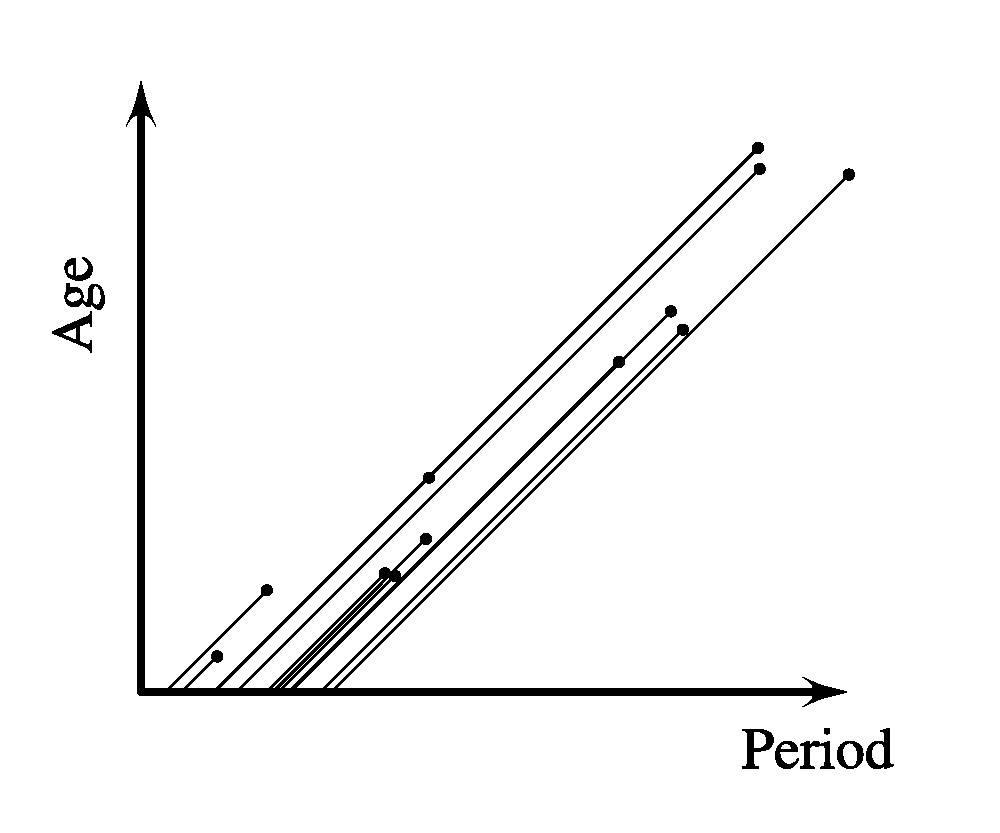
\includegraphics[width=\textwidth]{Figures/LexisSimplePlain1.pdf}}
\only<2>{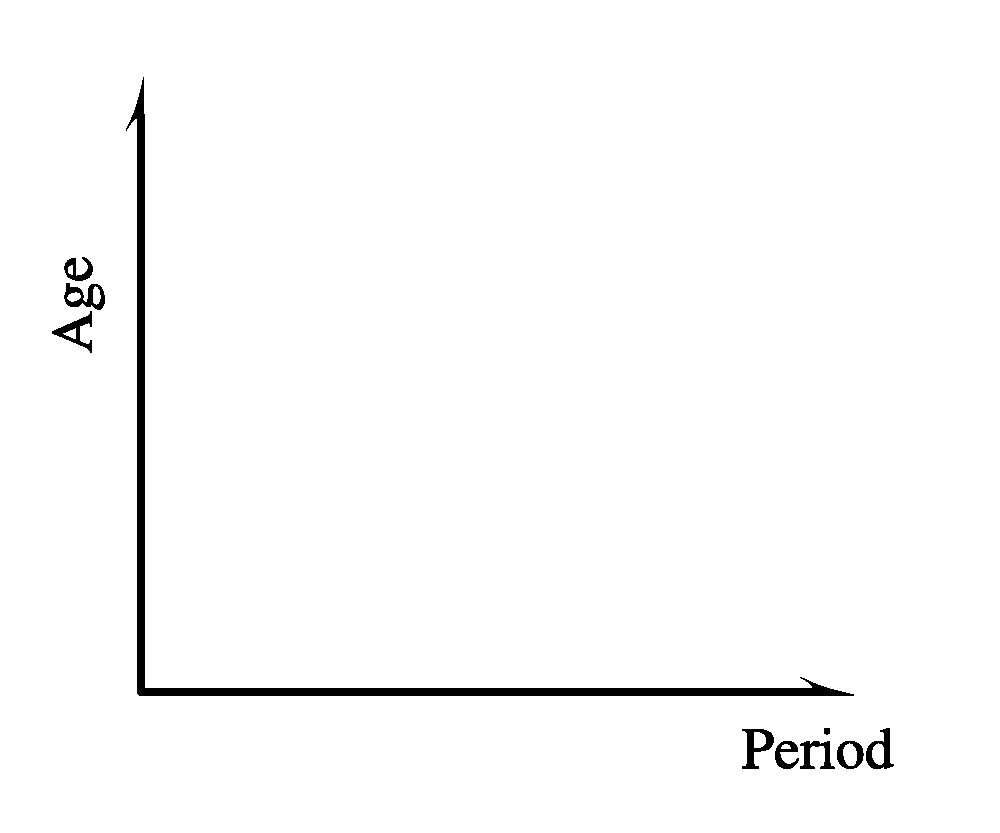
\includegraphics[width=\textwidth]{Figures/LexisSimplePlain2.pdf}}
\only<3>{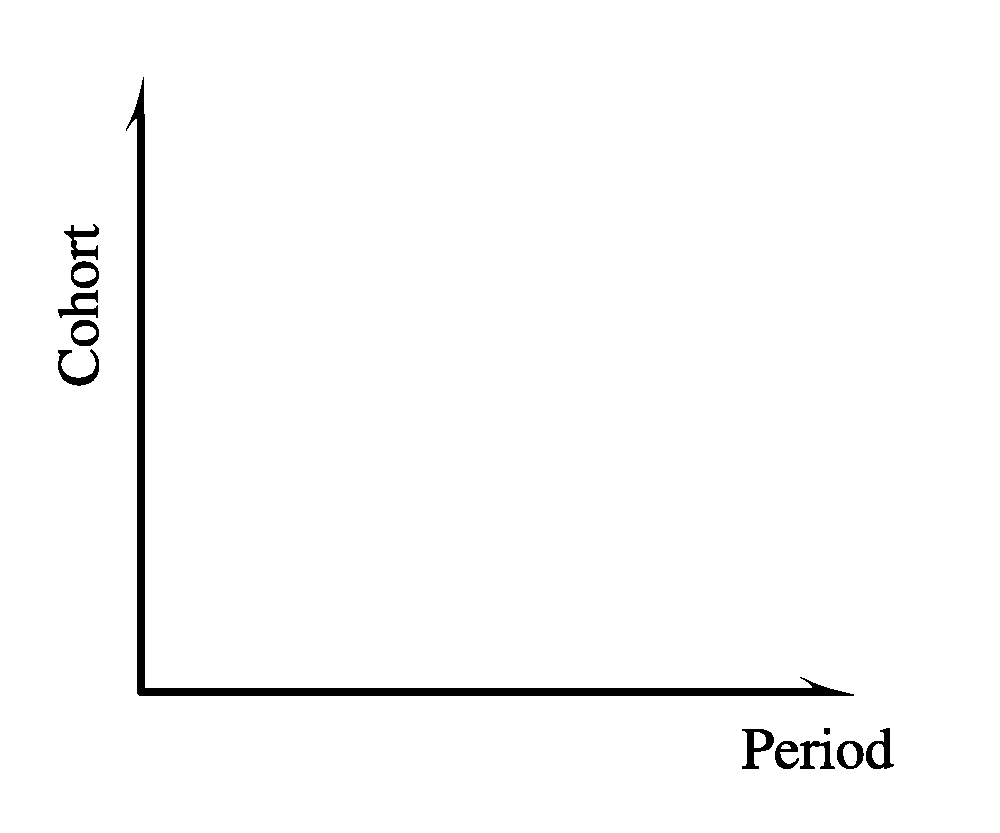
\includegraphics[width=\textwidth]{Figures/LexisSimplePlain3.pdf}}
\only<4>{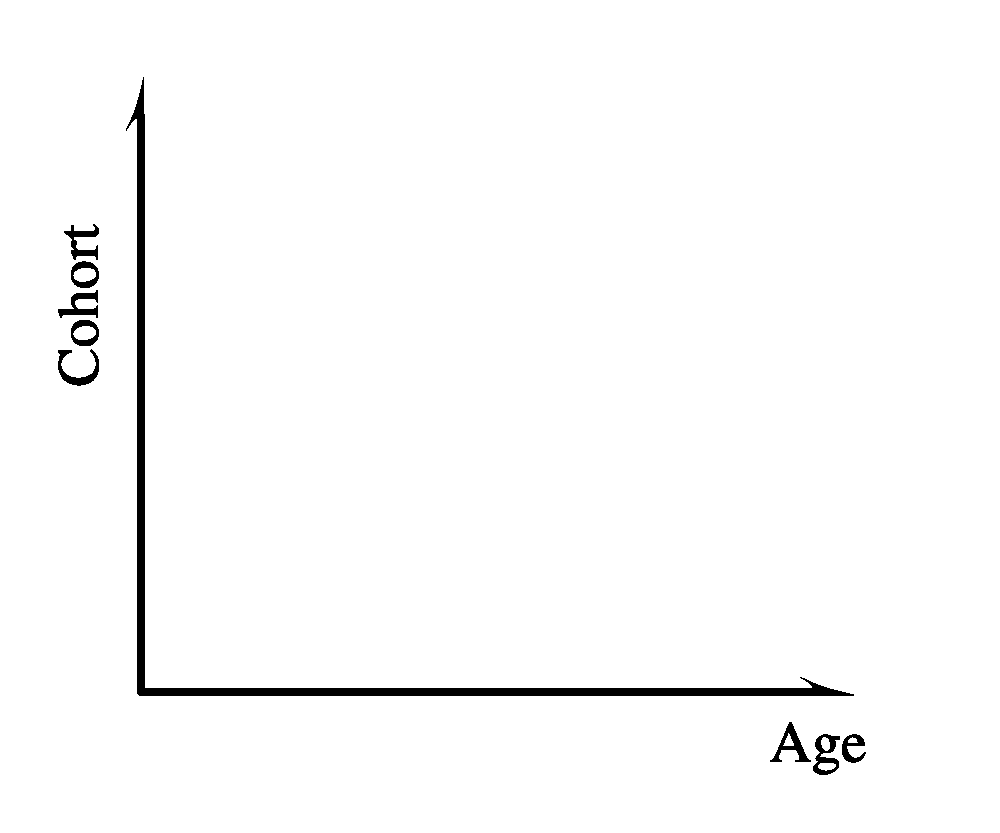
\includegraphics[width=\textwidth]{Figures/LexisSimplePlain4.pdf}}
\end{frame}

\begin{frame}[plain]
\begin{center}
\Large
Lexis' 3d marriage identity
\vspace{2em}

\includegraphics[scale=5]{Figures/LexisMarriageID.JPG}
\end{center}
\vspace{1em}
\small
Lexis (1875)
\end{frame}

\begin{frame}[plain]
\Large
\begin{center}
Lexis' 3d marriage identity
\vspace{1em}
\begin{itemize}
  \item Birth cohort
  \item Marriage cohort
  \item Separation cohort
  \item Age at marriage
  \item Age at separation
  \item Length of marriage
\end{itemize}
\end{center}
\end{frame}

%\begin{frame}[plain]
%\Large
%\begin{center}
%Riffe, et al. (2017) 3d identity
%\vspace{1em}
%\begin{itemize}
%  \item Birth cohort
 % \item Period
%  \item Time of death
%  \item Age
%  \item Time until death
%  \item Length of life
%\end{itemize}
%\end{center}

%\end{frame}

%---------------------------

\begin{frame}[plain]
\Large
\begin{center}
Brinks' (2014) 4d identity

\vspace{2em}
\includegraphics[scale=1.3]{Figures/Brinks2014.png}
\end{center}
\end{frame}

%-------------------
\newcolumntype{S}{ >{\centering\arraybackslash} m{2cm} }
\newcolumntype{D}{ >{\centering\arraybackslash} m{5.4cm} }
\newcolumntype{E}{ >{\centering\arraybackslash} m{3.7cm} }

\begin{frame}[plain]
\begin{center}
\begin{tabular}{S D}
dim & vec space \\
\hline
2 & 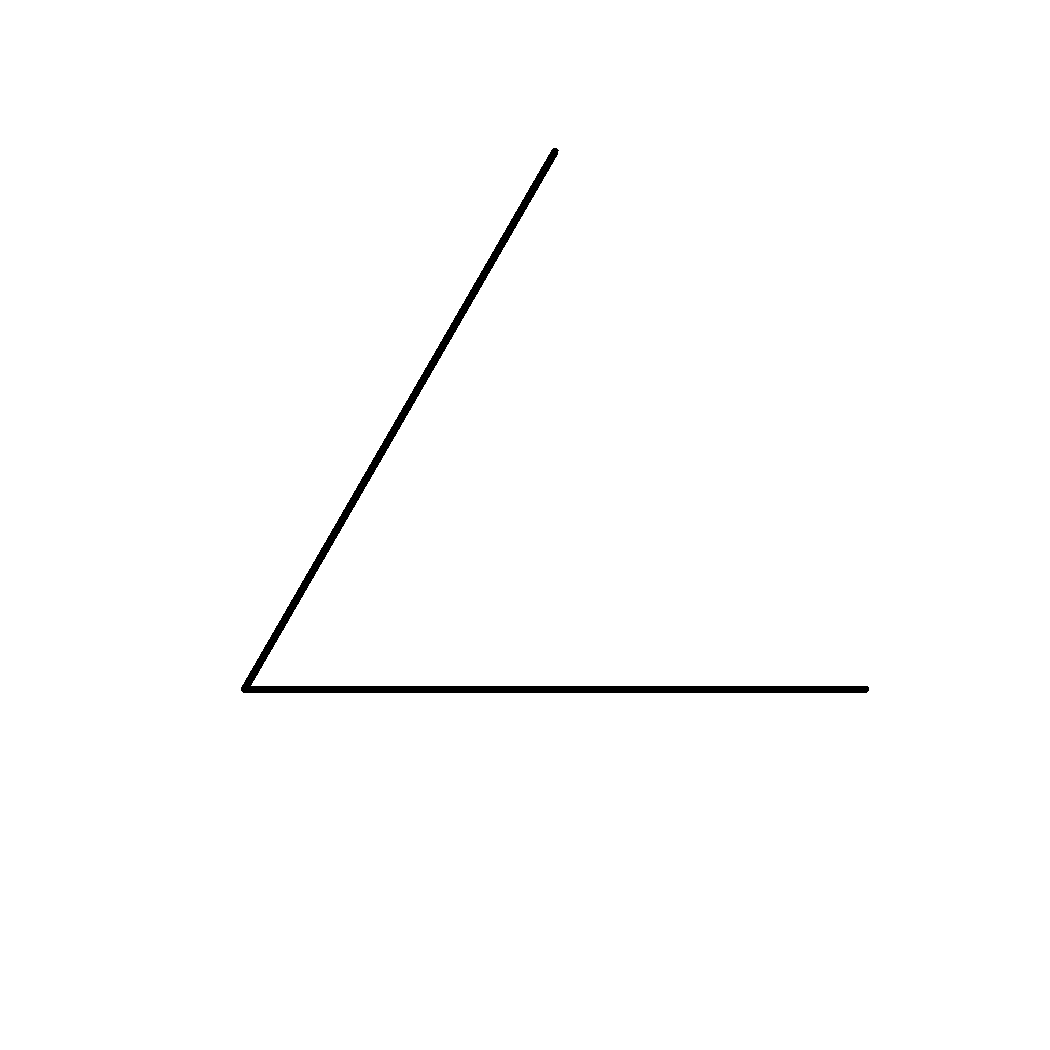
\includegraphics[scale=.3]{Figures/2dvec.pdf} \\
3 & 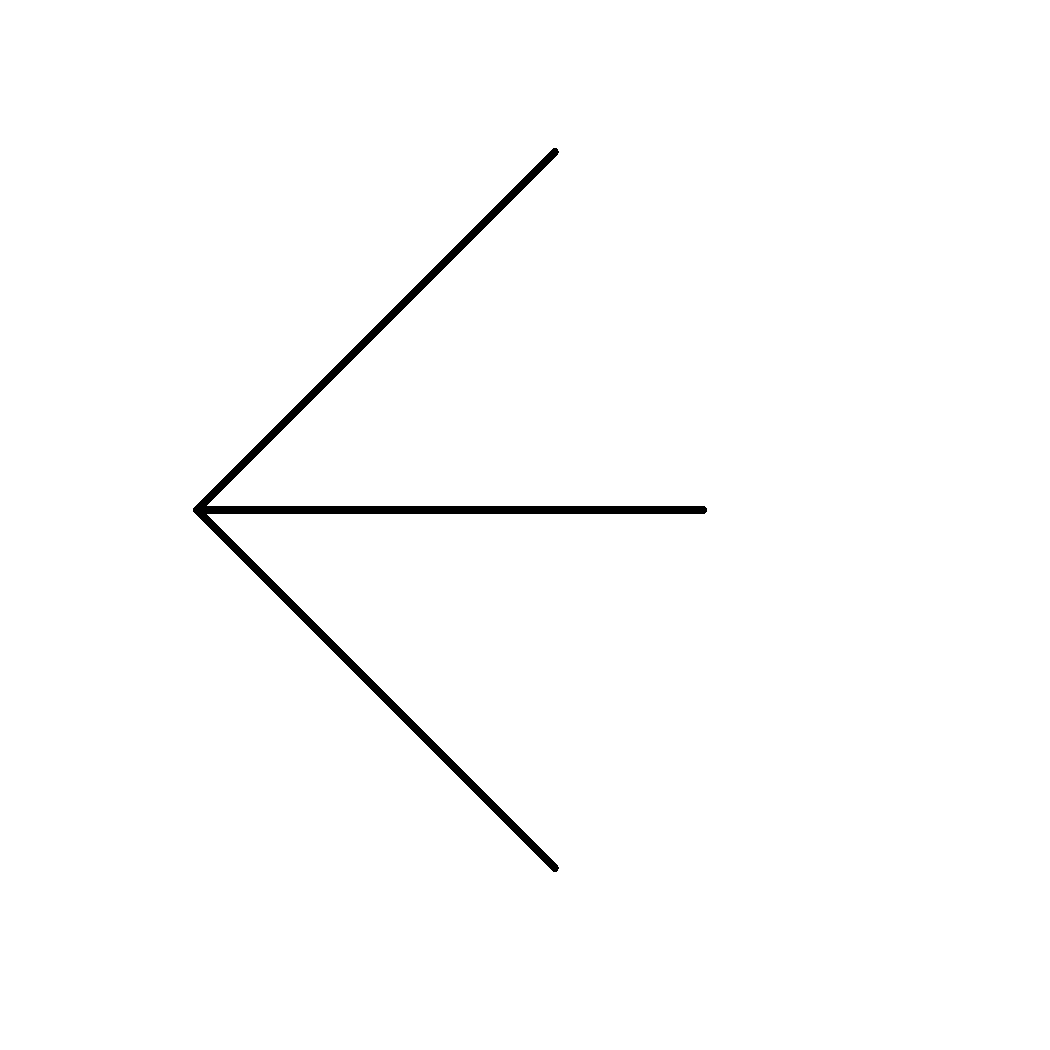
\includegraphics[scale=.3]{Figures/3dvec.pdf} \\
4 & 
\includegraphics[scale=.3]{Figures/4dvec.pdf} \\
\end{tabular}
\end{center}
\end{frame}

% ---------------------

\begin{frame}[plain]
\begin{center}
\begin{tabular}{S D}
dim & graph \\
\hline
2 & 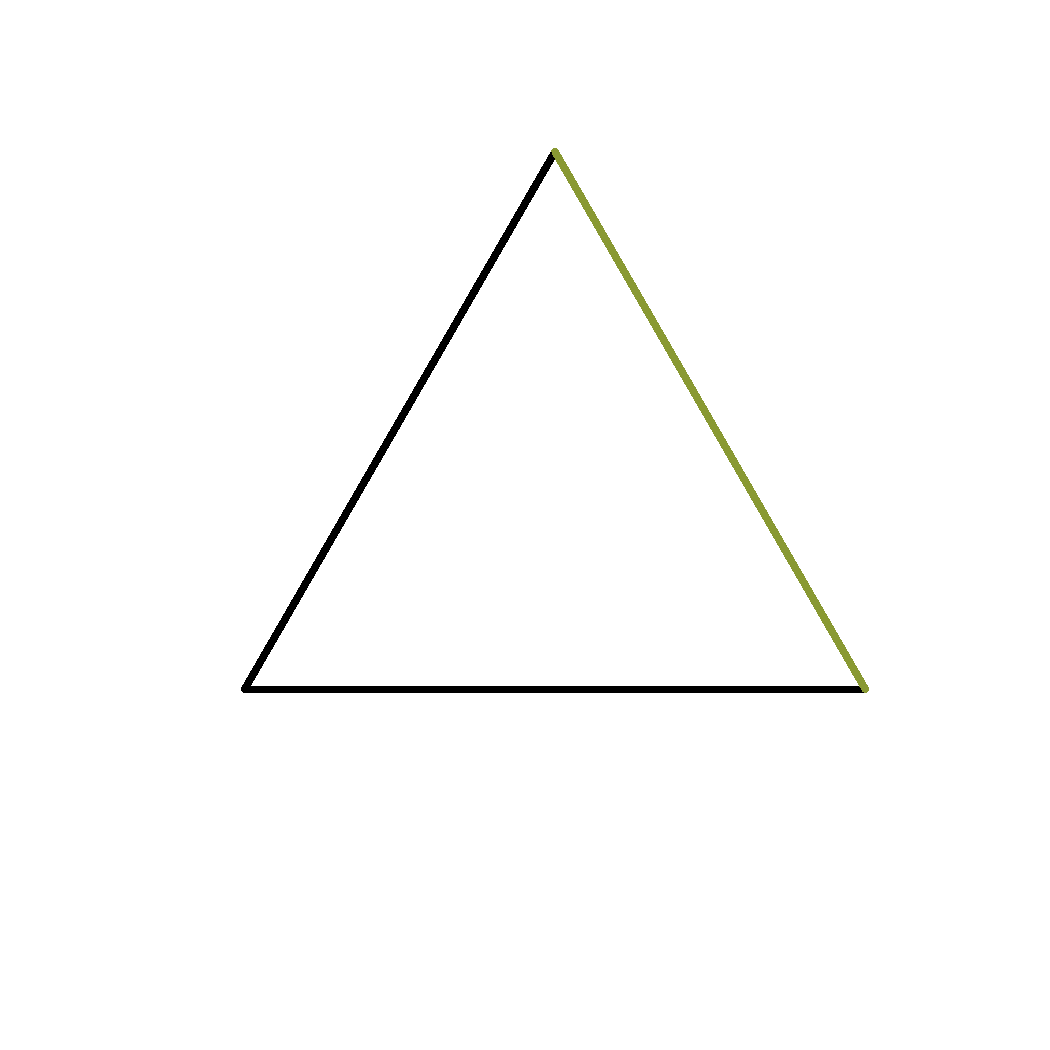
\includegraphics[scale=.3]{Figures/2dgraph.pdf} \\
3 & 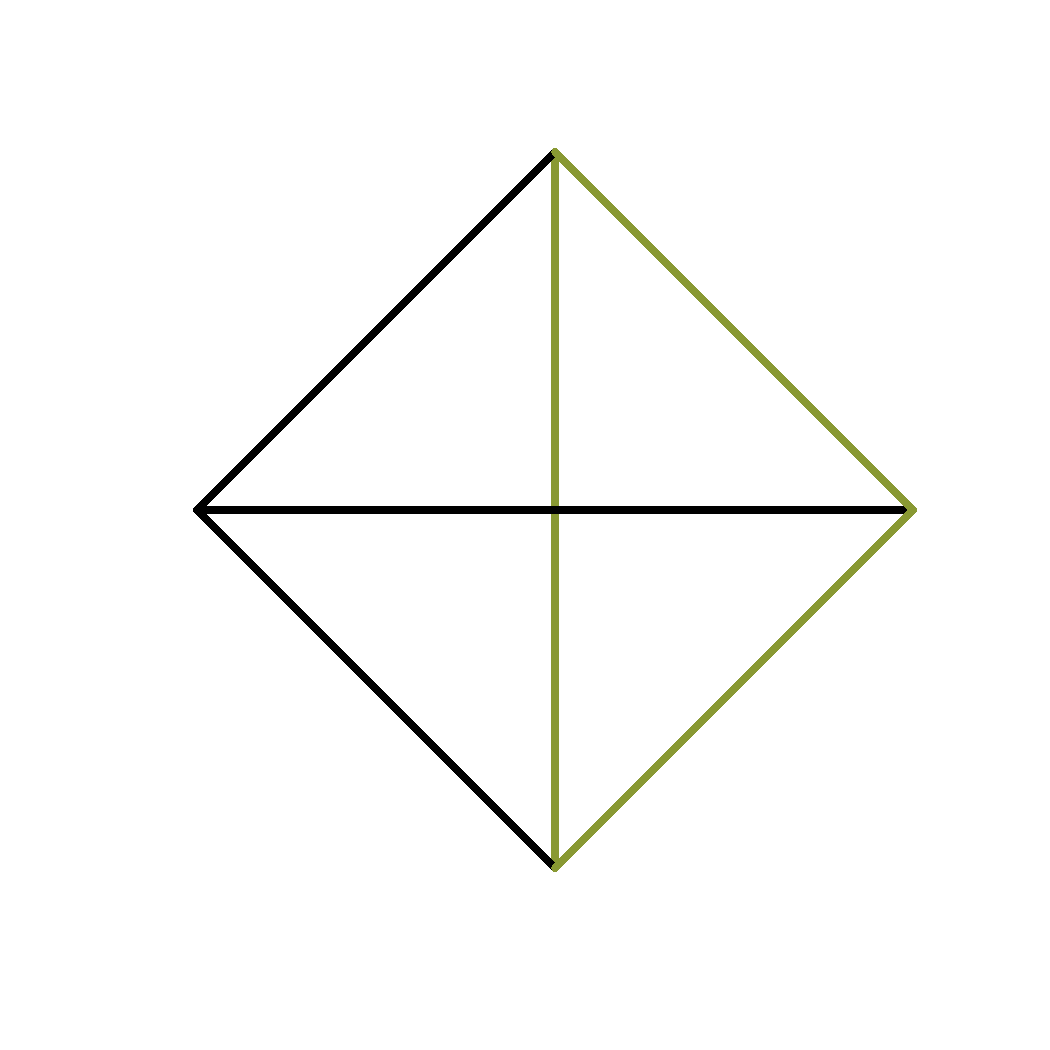
\includegraphics[scale=.3]{Figures/3dgraph.pdf} \\
4 & 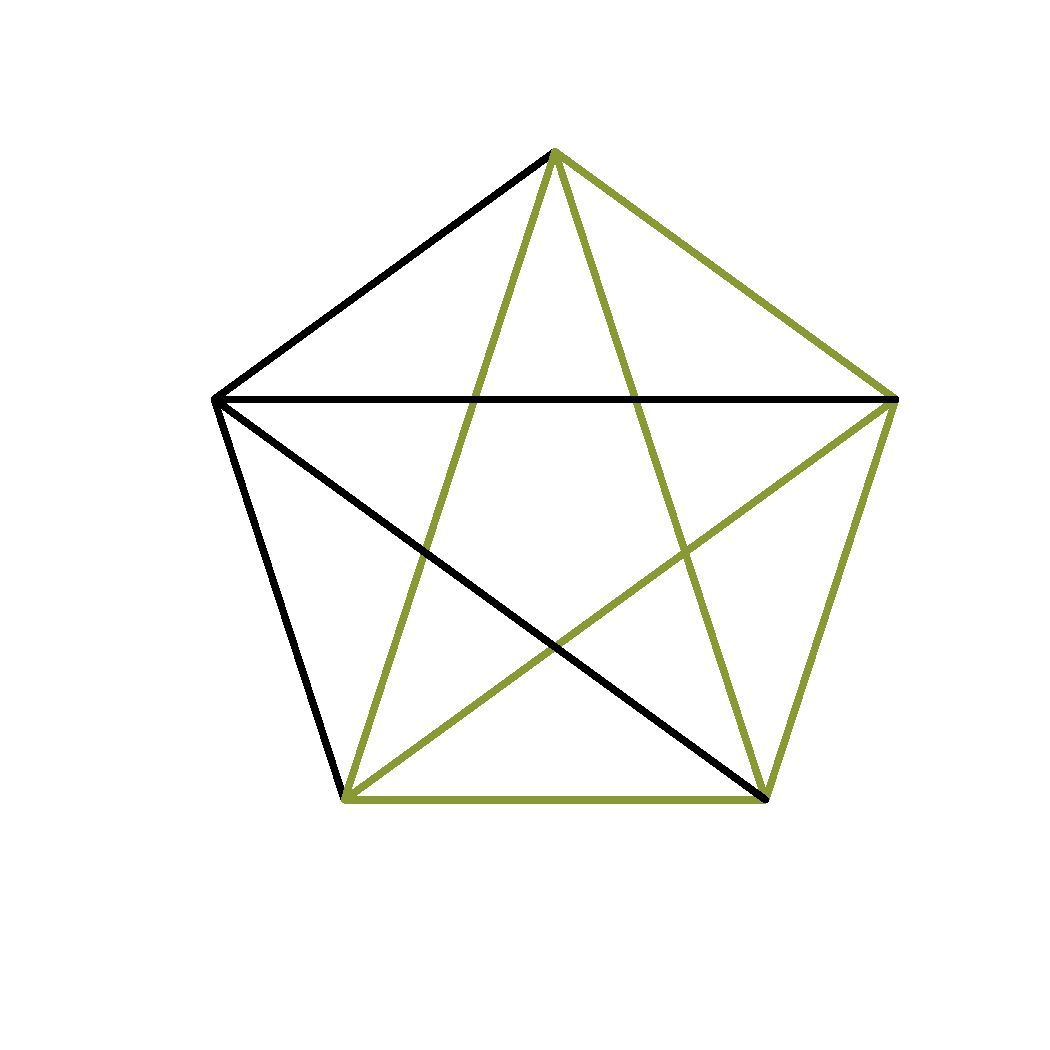
\includegraphics[scale=.3]{Figures/4dgraph.pdf} \\
\end{tabular}
\end{center}
\end{frame}

%-------------------

\begin{frame}[plain]
\Large
\begin{center}
Some thoughts on identification
\end{center}
\end{frame}

%-------------------

\begin{frame}[plain]
\begin{center}
\only<1>{
\includegraphics[scale=.9]{Figures/n2_1.pdf}}
\only<2>{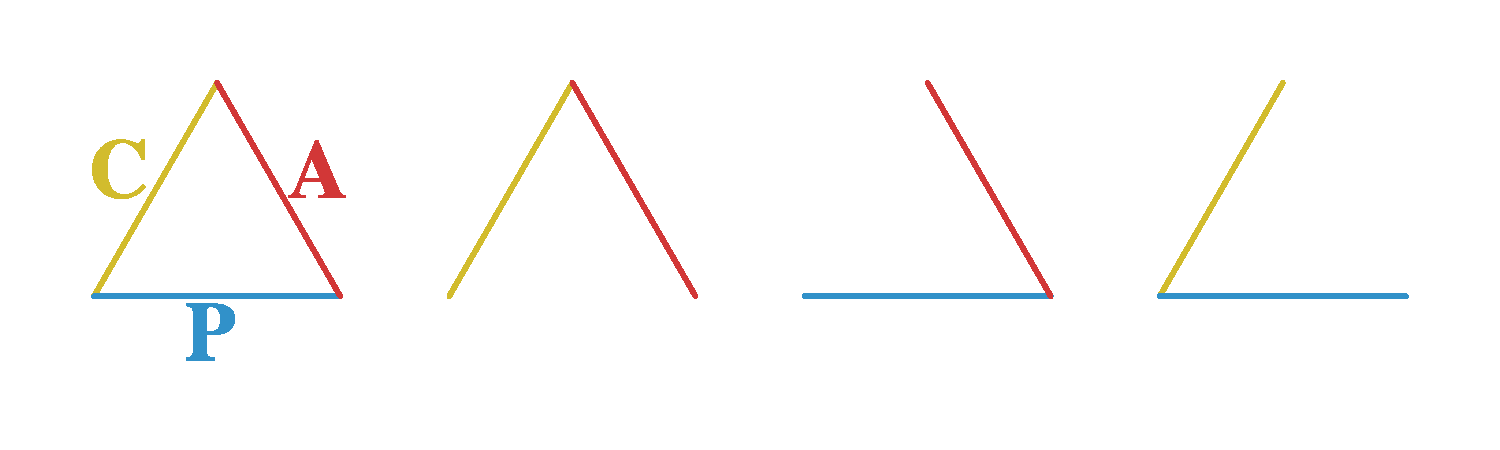
\includegraphics[scale=.9]{Figures/n2_2.pdf}}
\end{center}
\end{frame}

%-------------------

\begin{frame}[plain]
\Large
\begin{center}
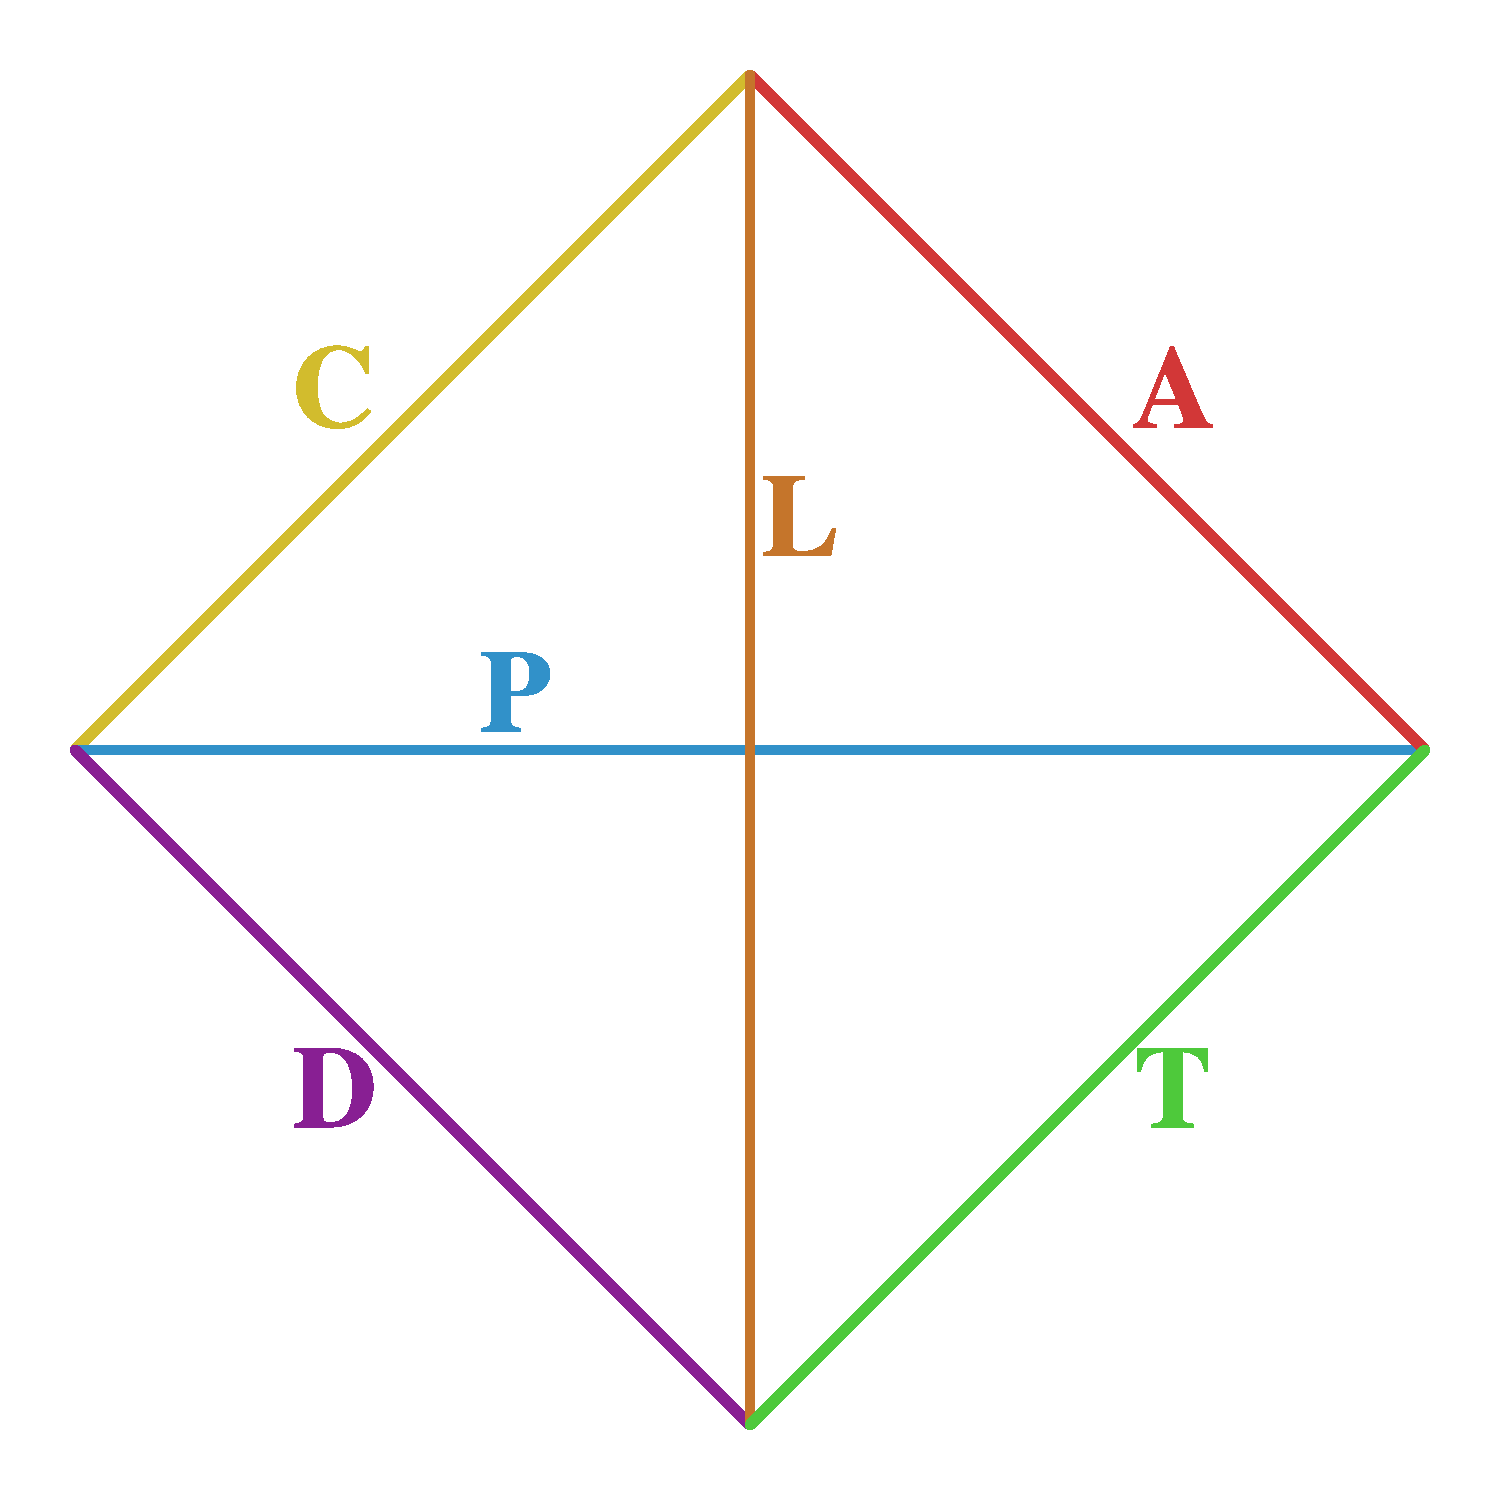
\includegraphics[scale=.7]{Figures/n3marked.pdf}
\end{center}
\end{frame}

%-------------------

\begin{frame}[plain]
\Large
\begin{center}
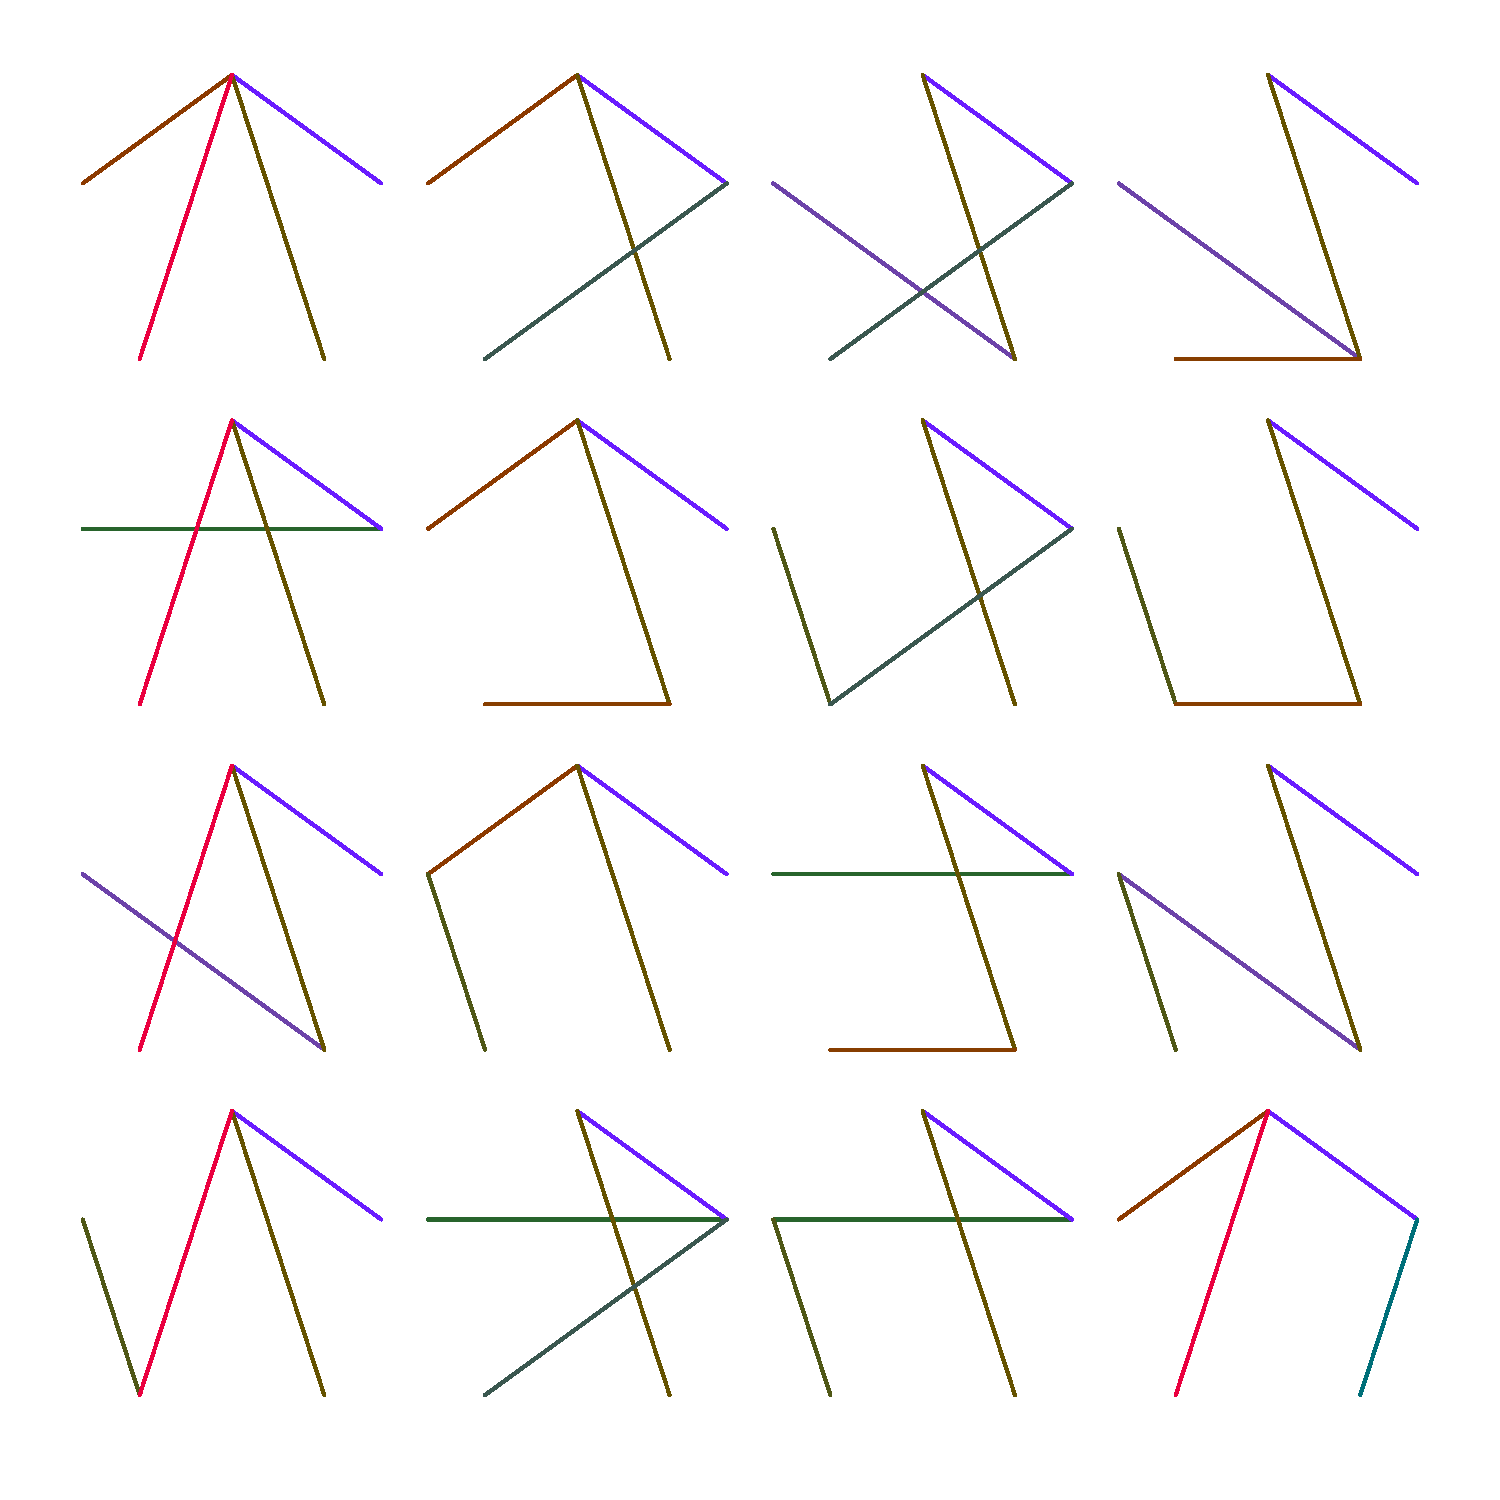
\includegraphics[scale=.7]{Figures/n3MST.pdf}
\end{center}
\end{frame}

%-------------------

\begin{frame}[plain]
\Large
\begin{center}
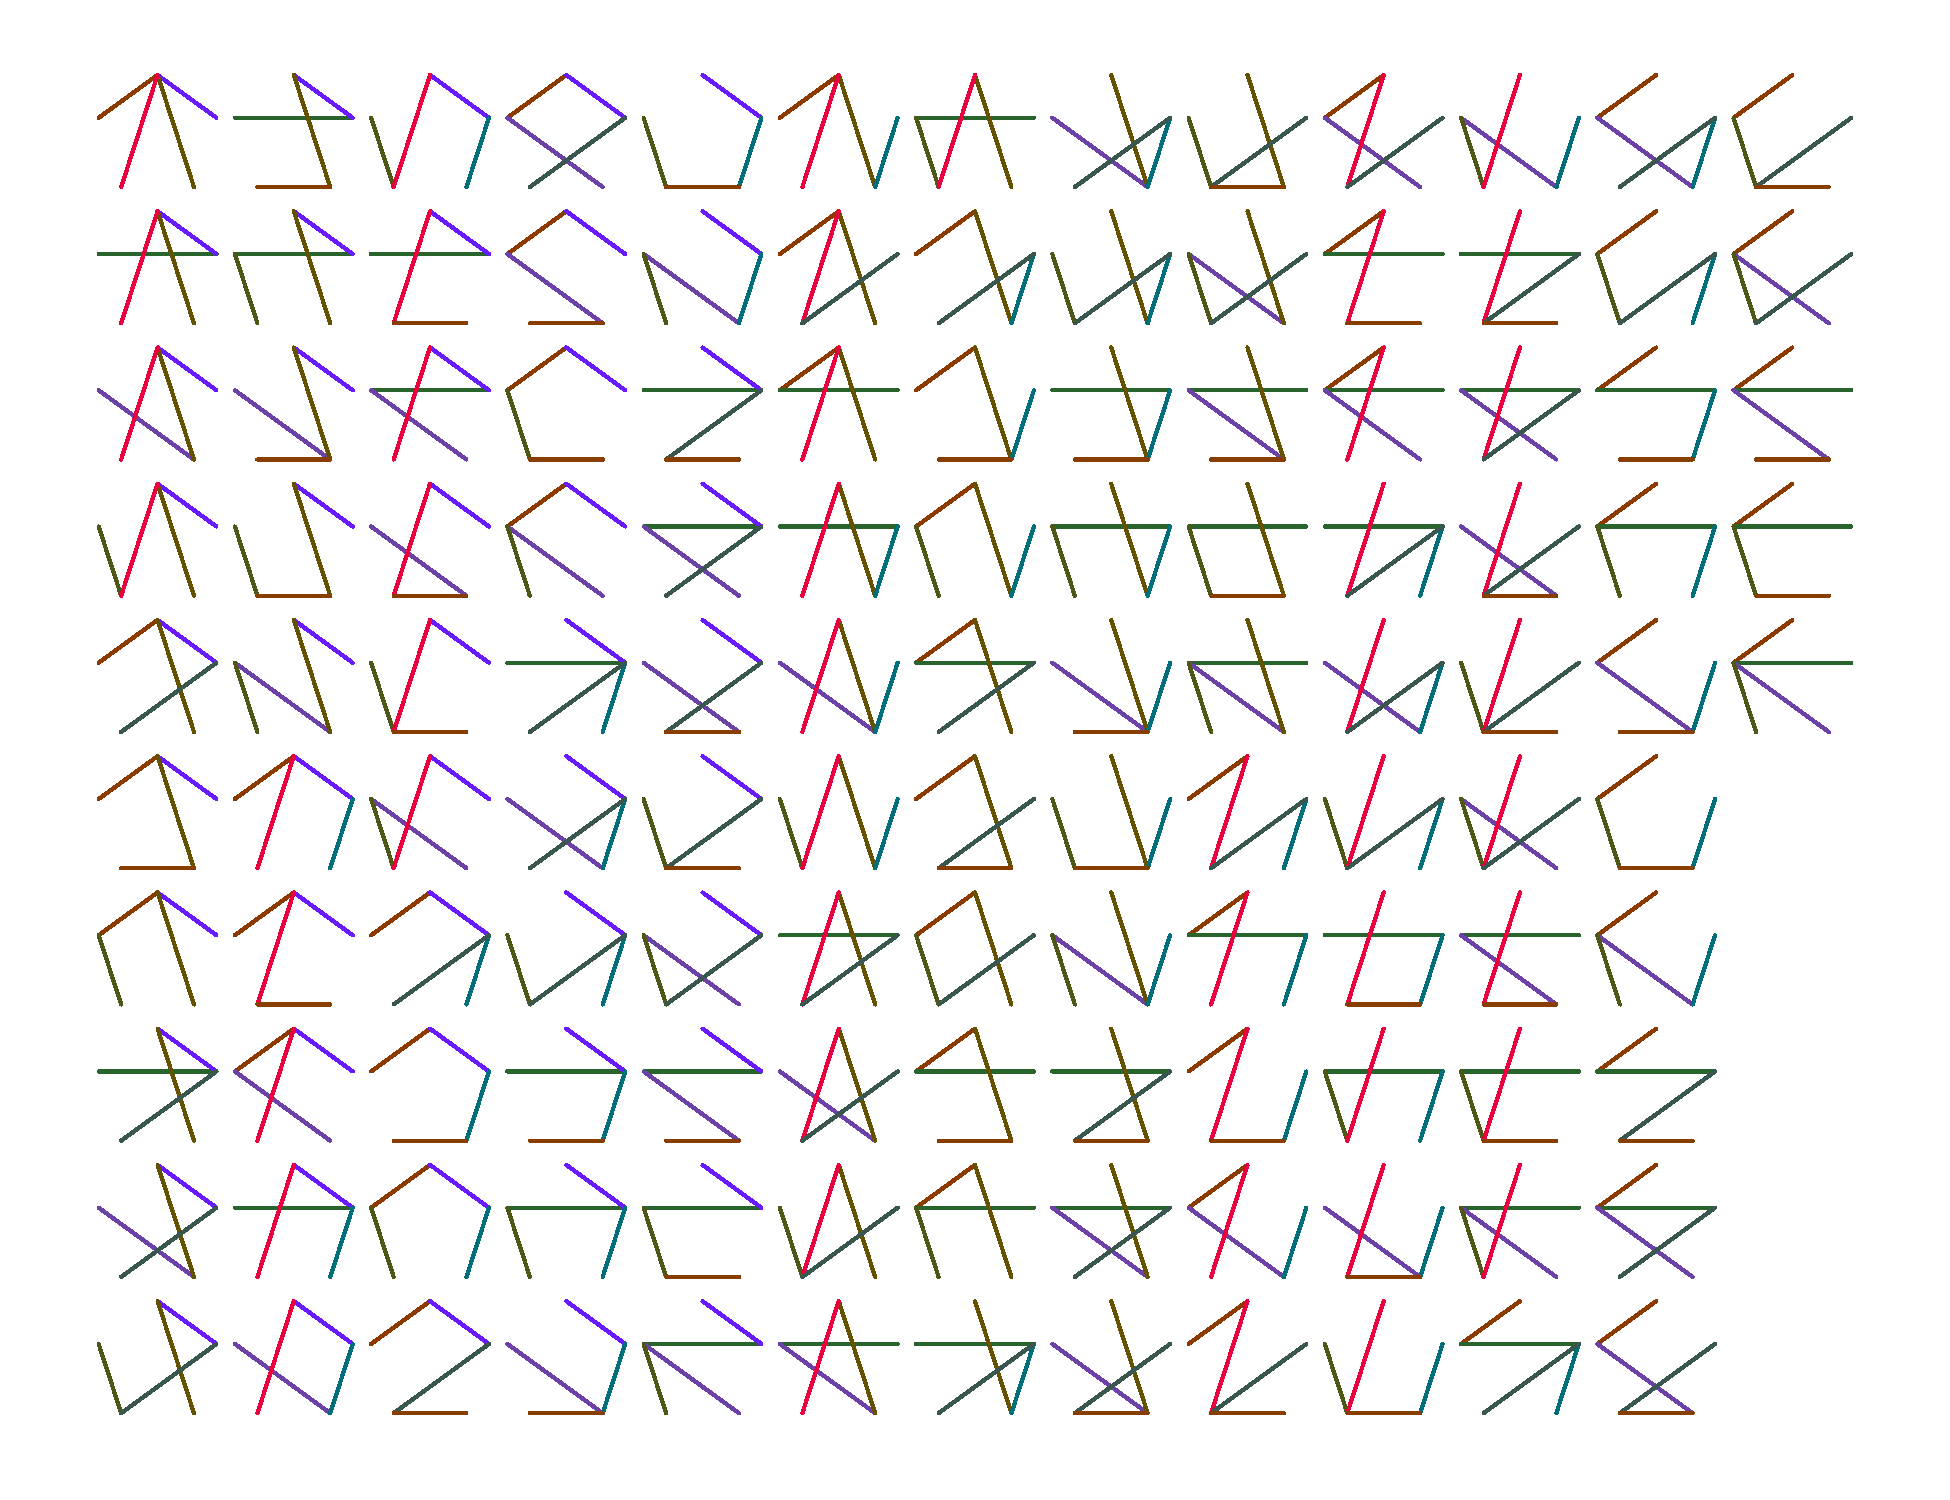
\includegraphics[scale=.7]{Figures/n4MST.pdf}
\end{center}
\end{frame}

%-------------------

\begin{frame}[plain]
\Large
\begin{center}
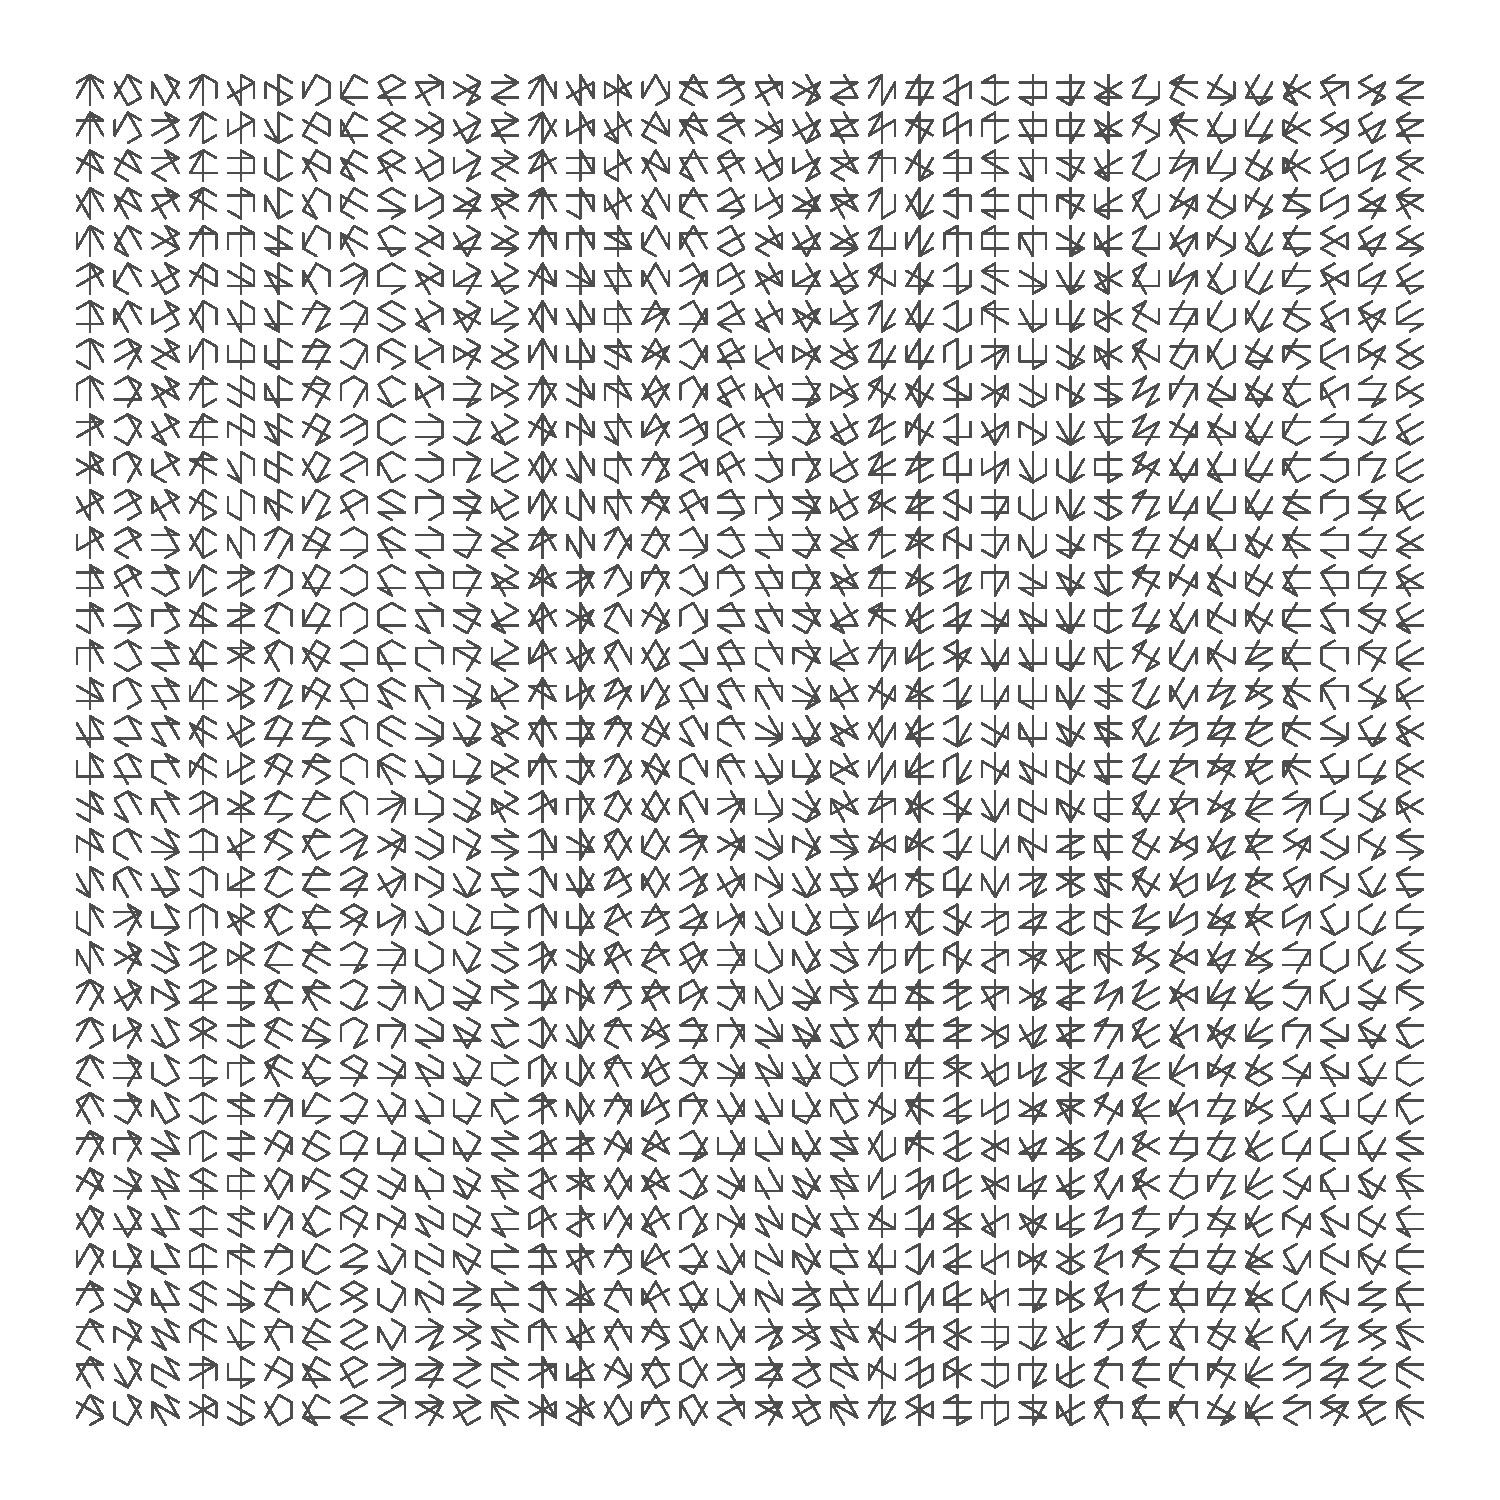
\includegraphics[scale=.7]{Figures/n5MST.pdf}
\end{center}
\end{frame}

%-------------------

\begin{frame}[plain]
\Large
\begin{center}

\includegraphics[scale=.7]{Figures/n6MST.pdf}
\end{center}
\end{frame}

%------------------

\begin{frame}[plain]
\Large
\begin{center}
\only<1>{So there's a lot you \emph{can} identify without nuance.}
\only<2>{Exactly $(n+1)^{(n-1)}$ MSTs on n events.}
\only<3>{And $\binom{n+1}{3}$ 2d simplices in an $n$-dimensional temporal
identity.}
\end{center}
\end{frame}

%------------------

\begin{frame}[plain]
\only<1>{\includegraphics[width=23cm]{Figures/APCtimeline.JPG}}
\only<2>{\includegraphics[width=23cm]{Figures/APCtimeline2.png}}
\only<3>{\includegraphics[width=23cm]{Figures/APCtimeline3.png}}
\end{frame}

%-------------------

\begin{frame}[plain]
\Large
\begin{center}
Events and durations are key.
\end{center}
\end{frame}

%-------------------

\begin{frame}[plain]
\Large
\begin{center}
\only<1>{Events determine dimensionality.}
\only<2>{Events are either \emph{anchored} in time or calendar breadcrumbs:
\emph{period}.} 
\only<3>{Event types determine duration types: \emph{fixed} or
\emph{scaling}.}
\only<4>{The combination of these four types of time measures imply four
different kinds of 2d identities.} 
\end{center}
\end{frame}

% -----------------

\begin{frame}[plain]
% something on classes of subidentities
\Large
\begin{center}
\includegraphics[height=12cm]{Figures/Composition3.png}

A 4-event identity
\end{center}
\end{frame}

%-------------------

\begin{frame}[plain]
\begin{center}
\only<1>{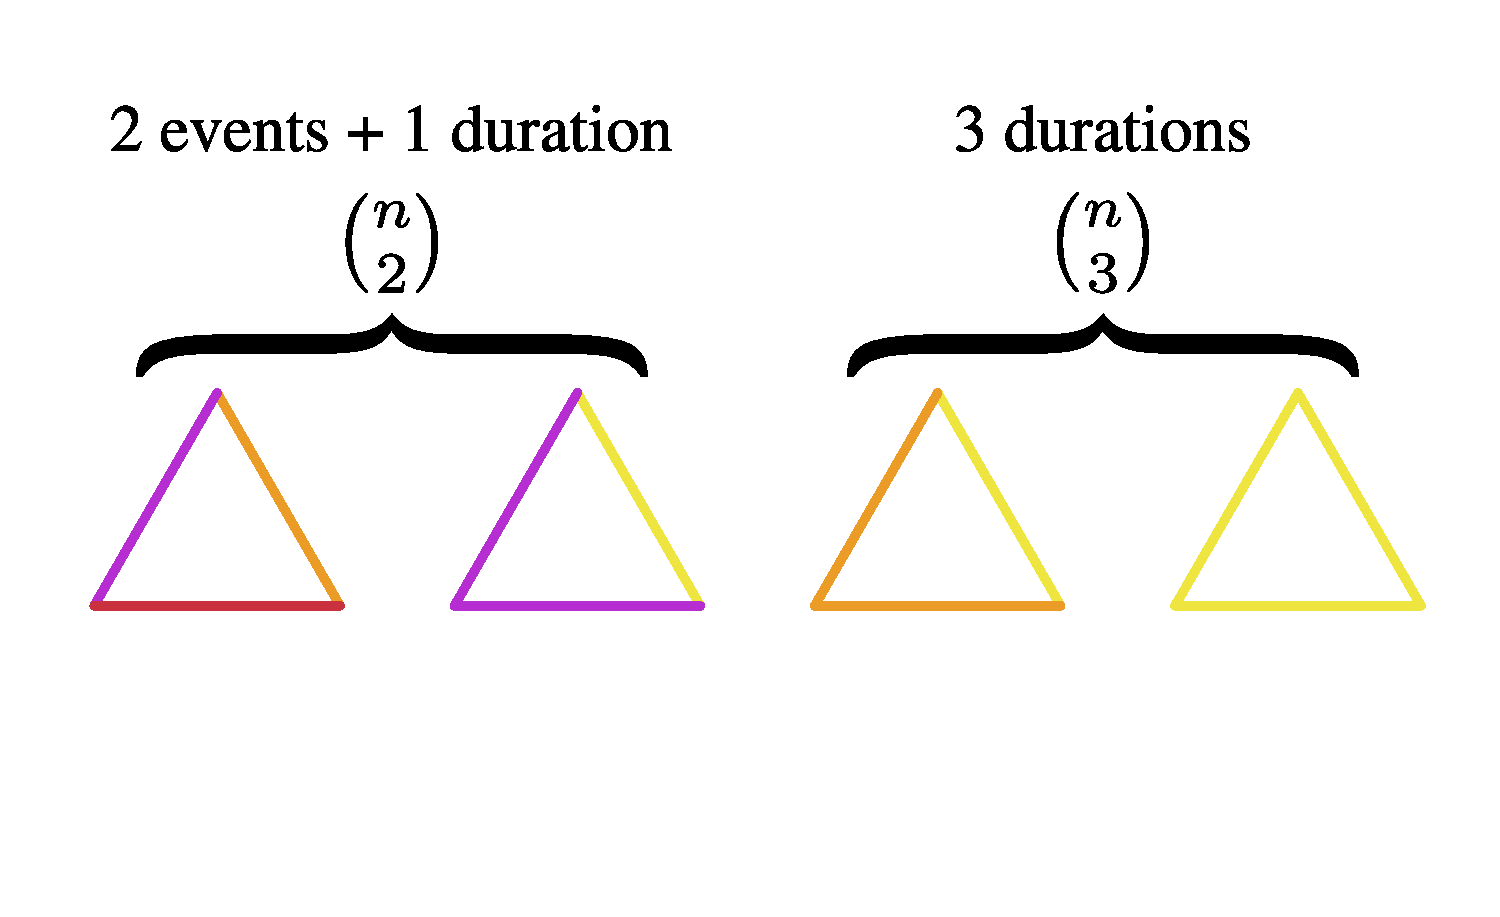
\includegraphics[scale=.9]{Figures/id3types1.pdf}}
\only<2>{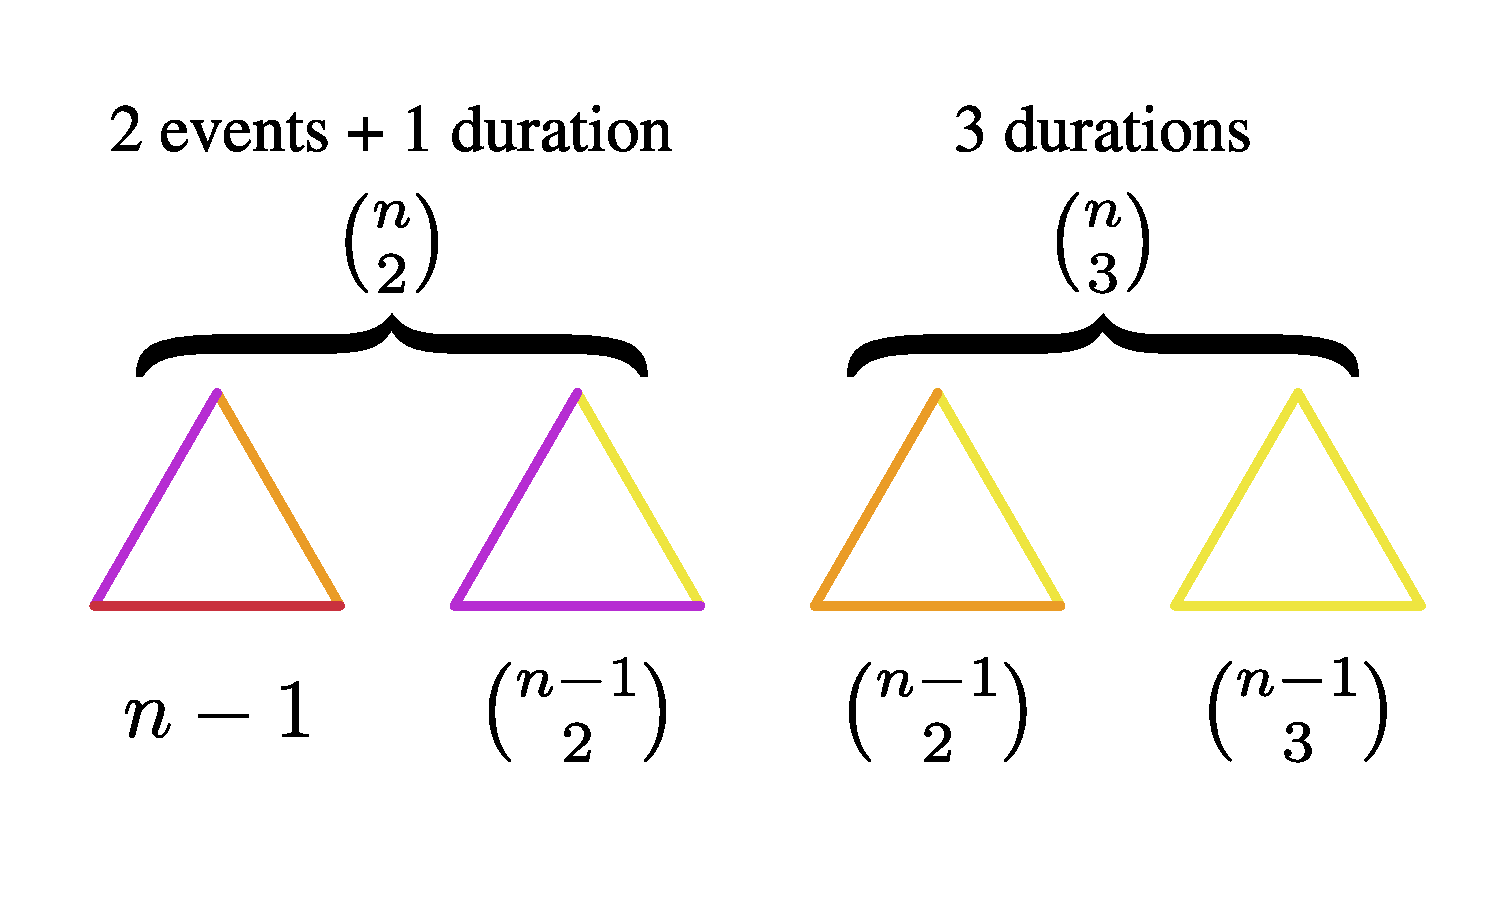
\includegraphics[scale=.9]{Figures/id3types2.pdf}}
\only<3>{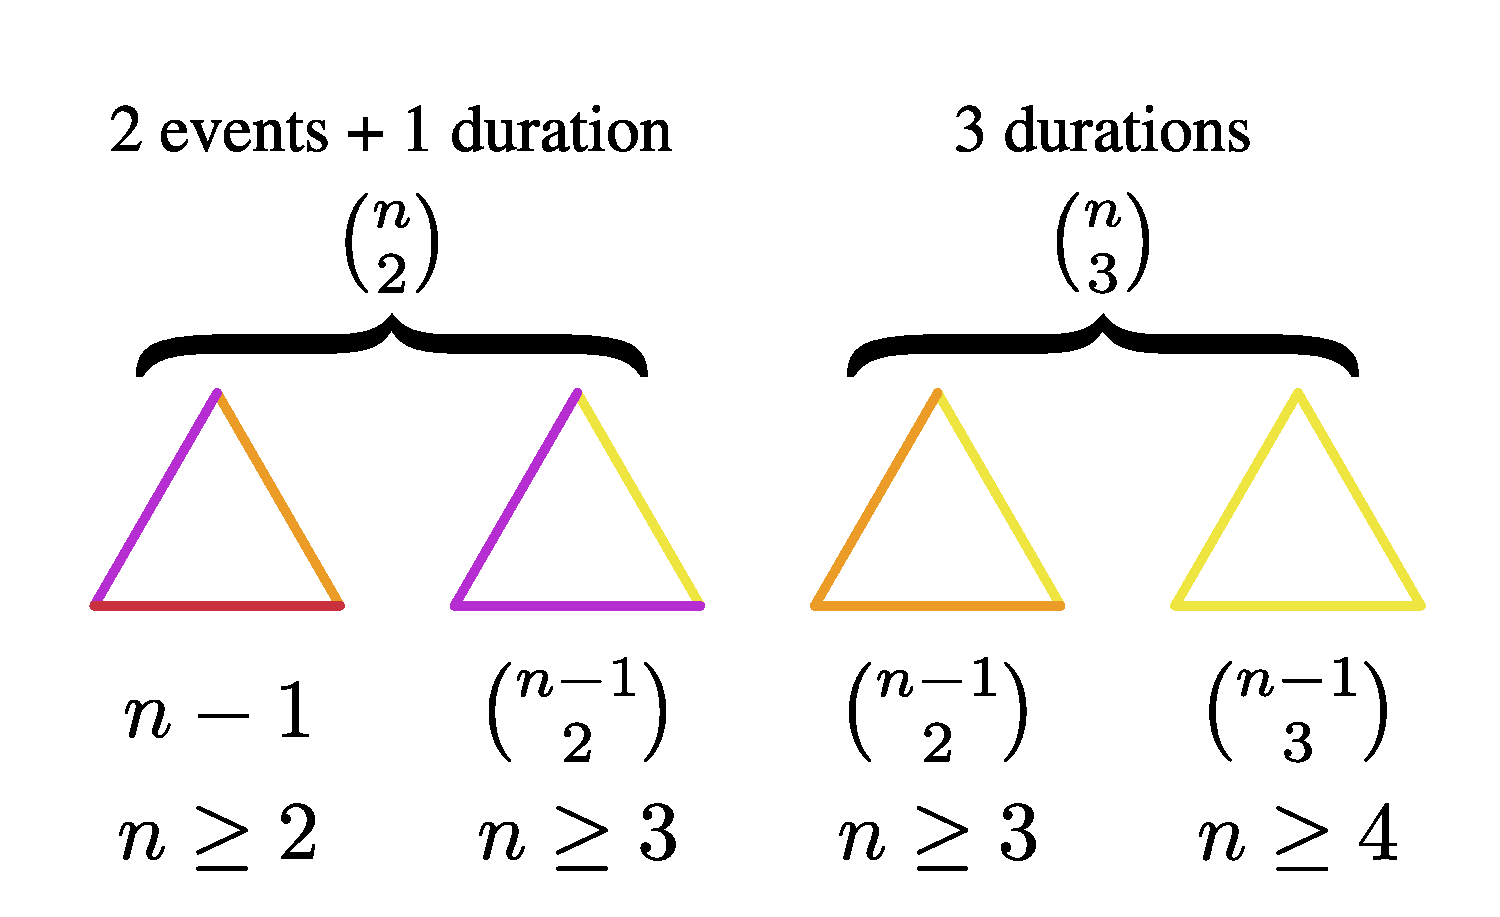
\includegraphics[scale=.9]{Figures/id3types3.pdf}}
\end{center}
\end{frame}

% -----------------

\begin{frame}[plain]
% something on classes of subidentities

\begin{center}
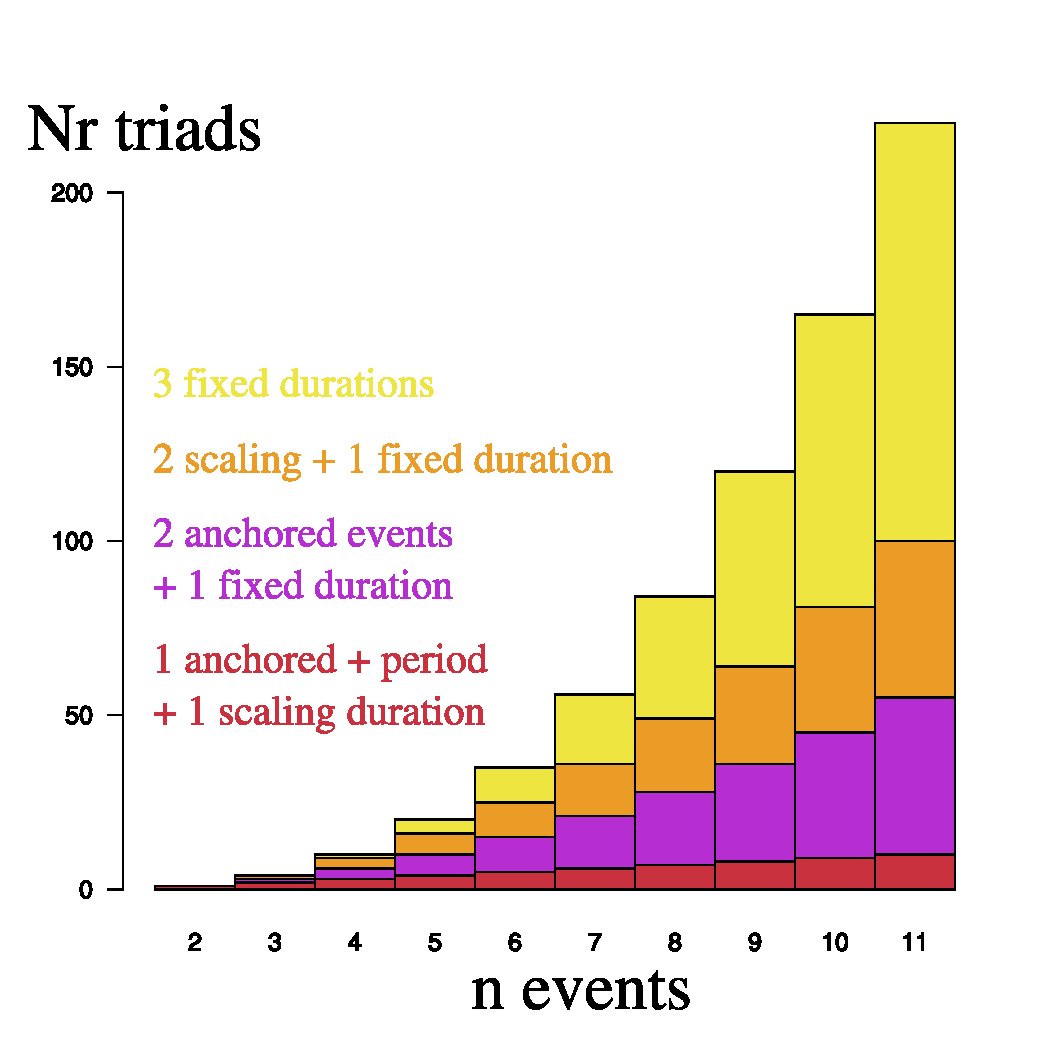
\includegraphics[scale=1]{Figures/id3compmarked.pdf}
\end{center}

\end{frame}

% -----------------



\begin{frame}
\Large
\begin{center}

  \begin{center}
        \begin{tikzpicture}
            \node[anchor=south west,inner sep=0] (image) at (0,0)
            {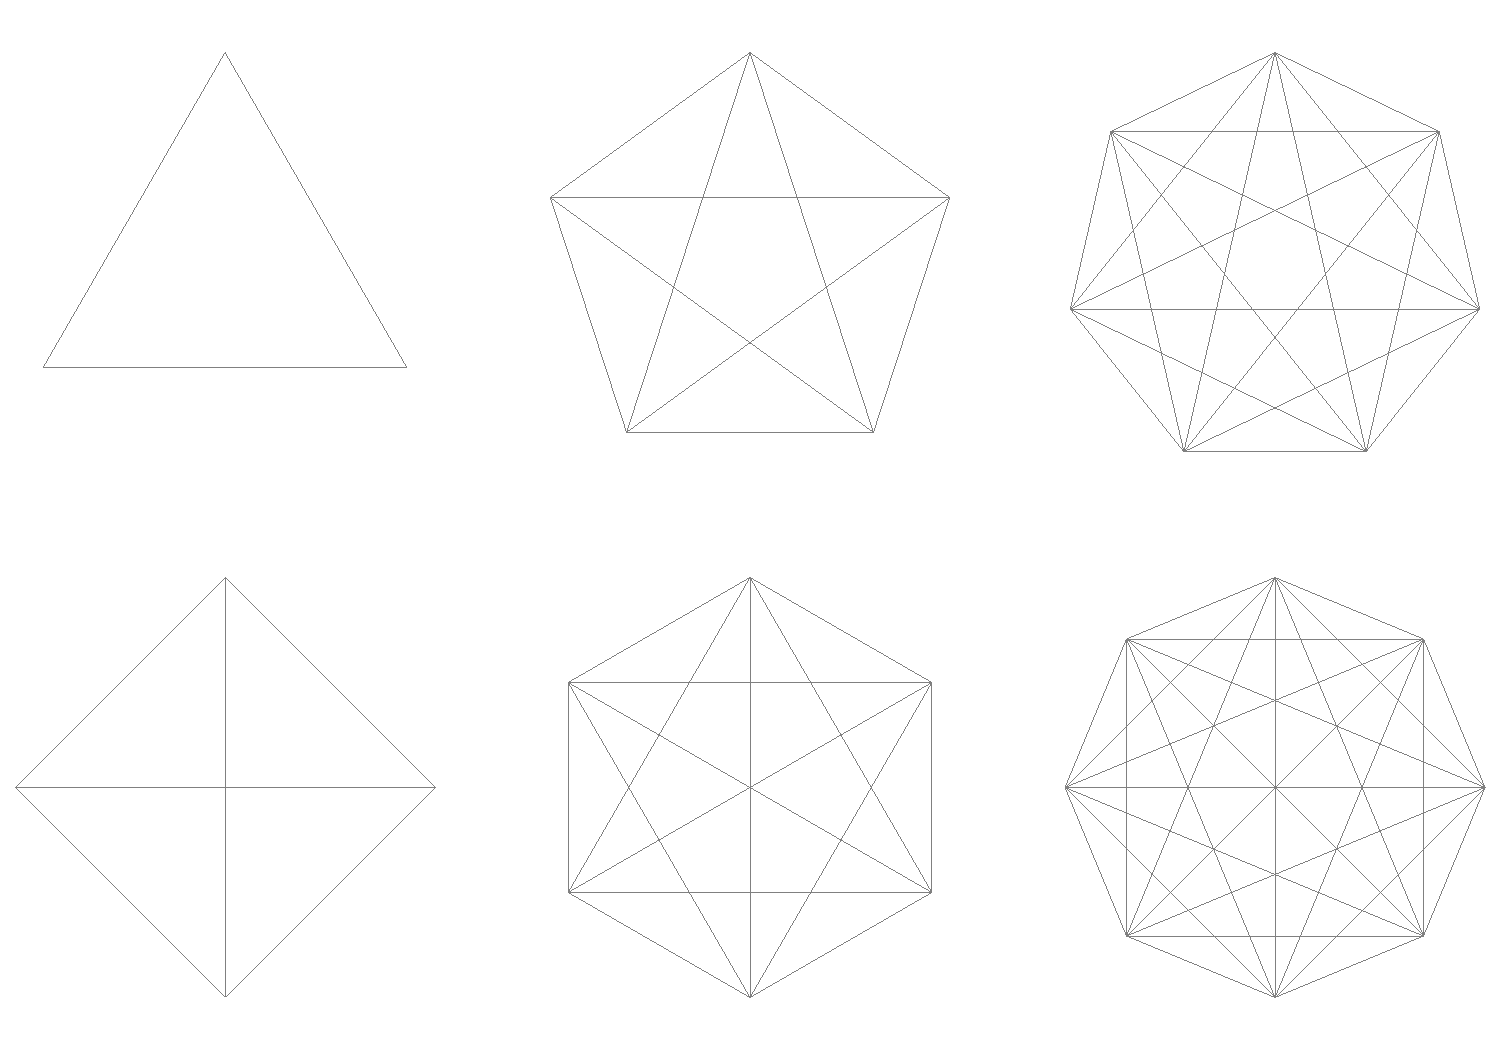
\includegraphics[width=1\textheight]{Figures/n2_7.pdf}}; \node[align=center,font={\Huge\bfseries}] at (image.center) {Thanks!\\
riffe@demogr.mpg.de};
        \end{tikzpicture}
    \end{center}

\end{center}

\end{frame}
%%%%%%%%%%%%%%%%%%%%%%%%%%%%%%%%%%
%%	End of the document			%%
%%%%%%%%%%%%%%%%%%%%%%%%%%%%%%%%%%
\end{document}










